\section{Taylorpolynom und Taylorentwicklung}

\begin{figure}[h]
	\centering
	\begin{subfigure}[b]{0.3\textwidth}
		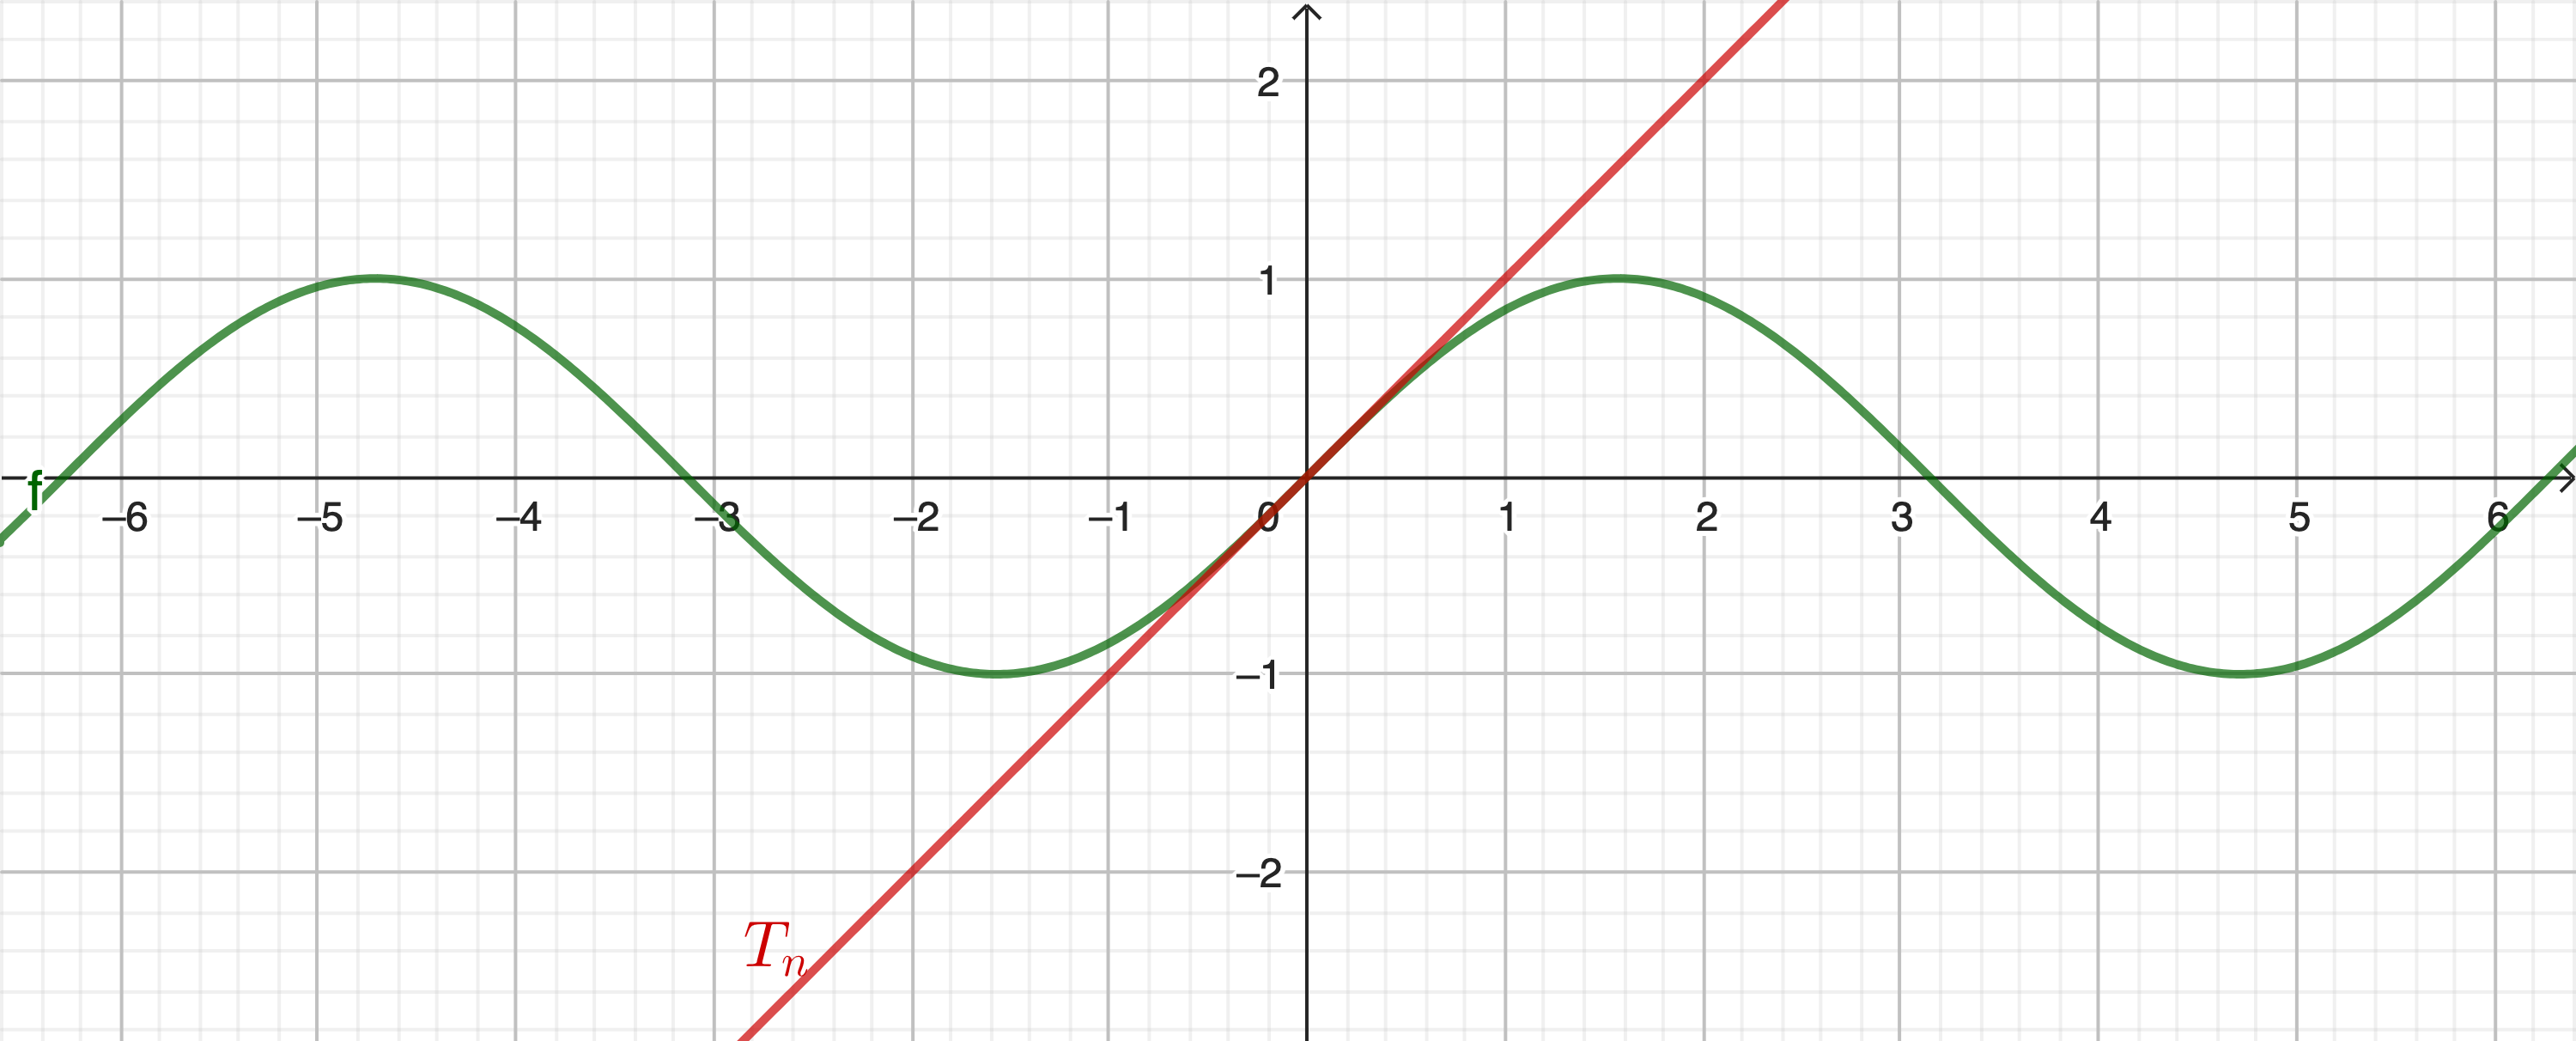
\includegraphics[width=\textwidth]{media/SinusT1.png}
		\caption*{Approximation durch ein Polynom von Grad 1}
	\end{subfigure}
	\begin{subfigure}[b]{0.3\textwidth}
		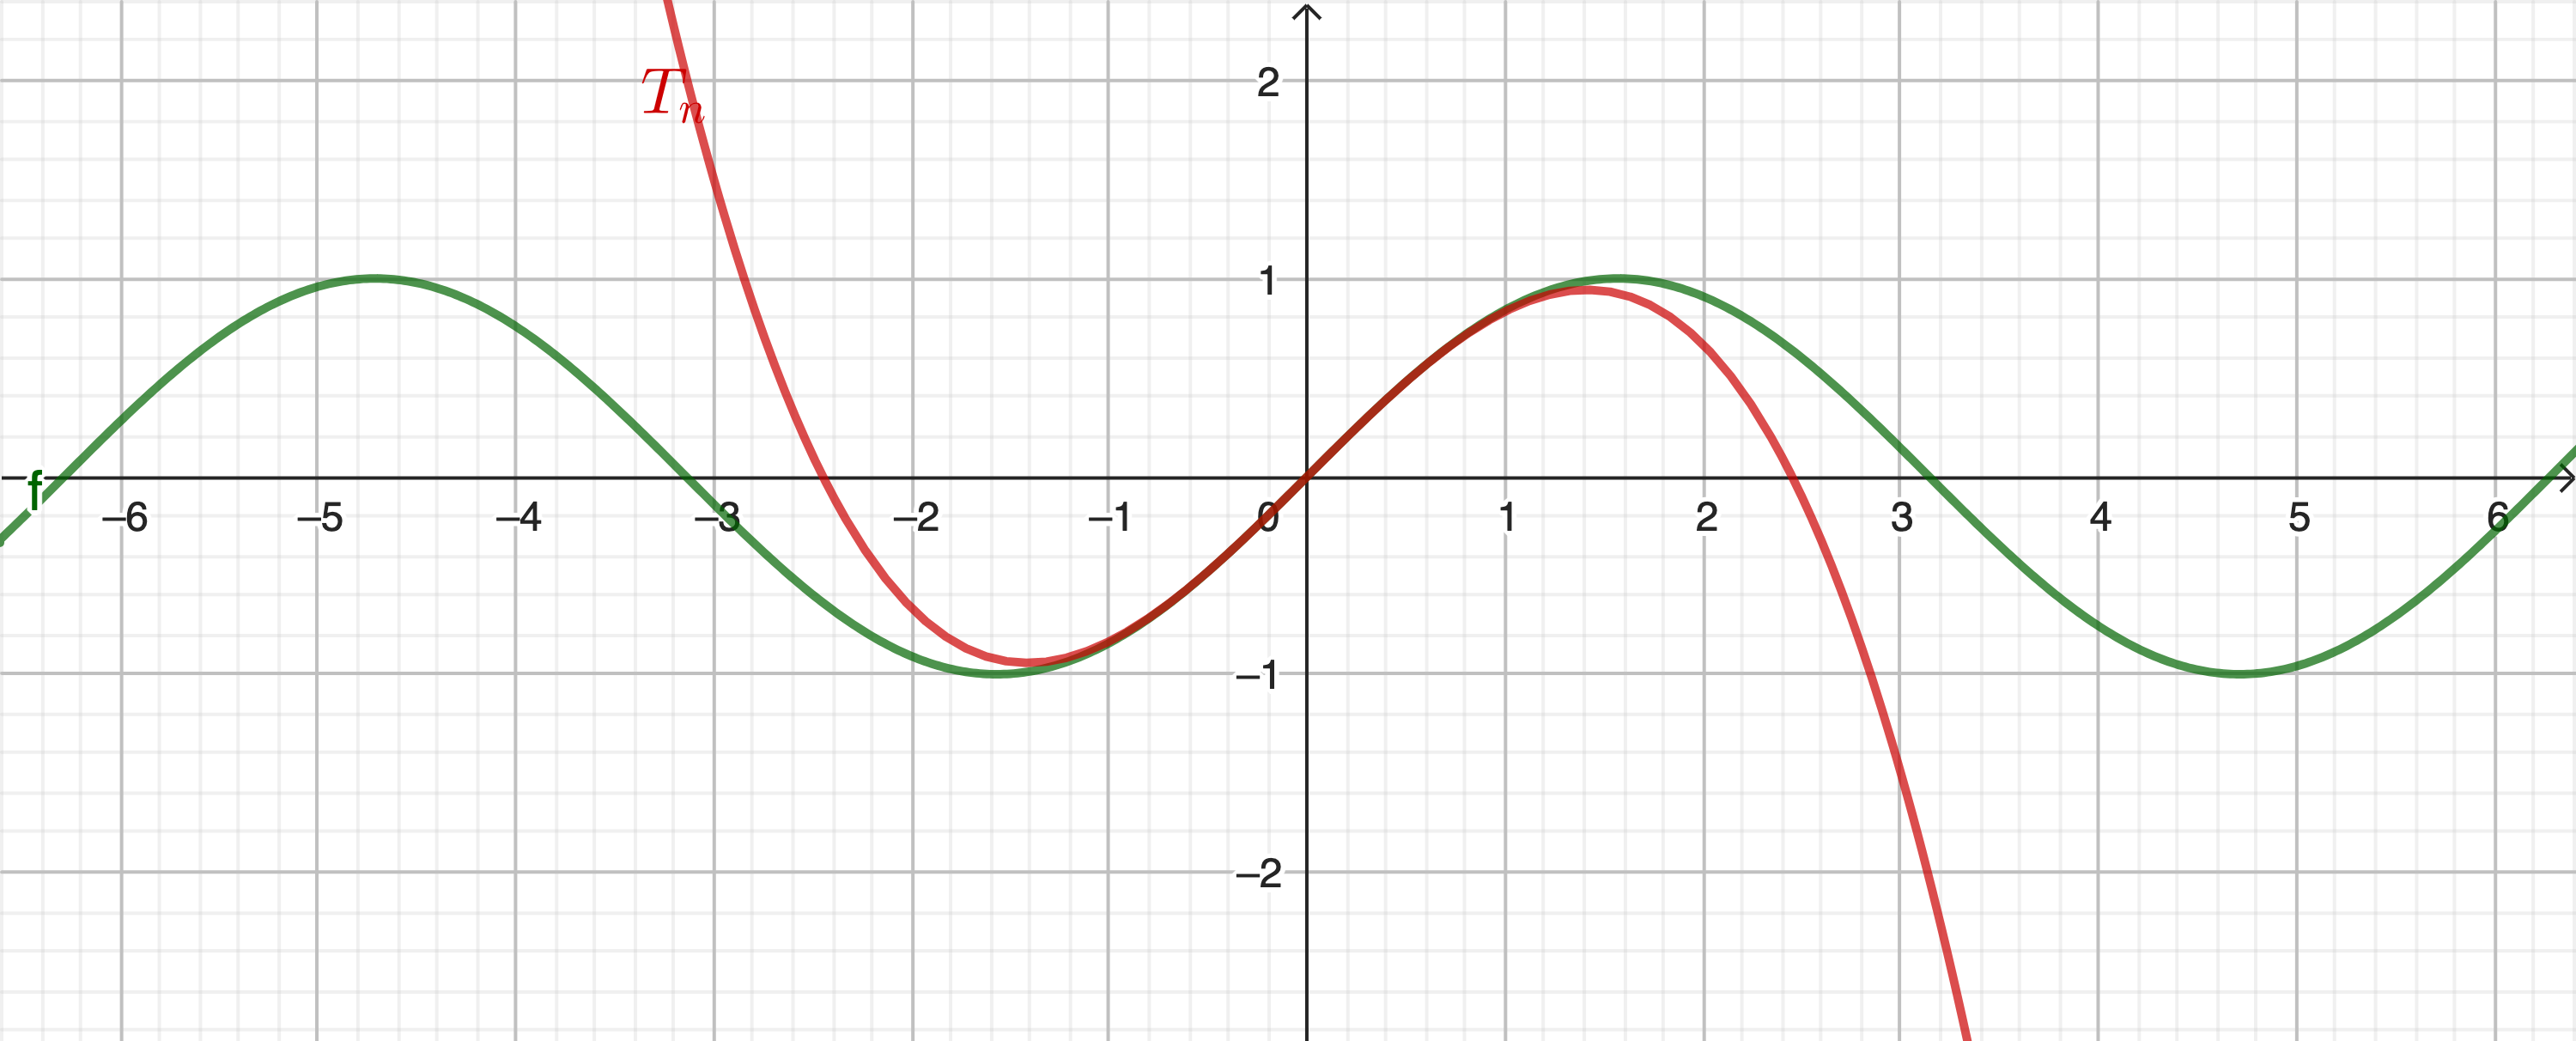
\includegraphics[width=\textwidth]{media/sinusT3.png}
		\caption*{Approximation durch ein Polynom von Grad 3}
	\end{subfigure}
	\begin{subfigure}[b]{0.3\textwidth}
		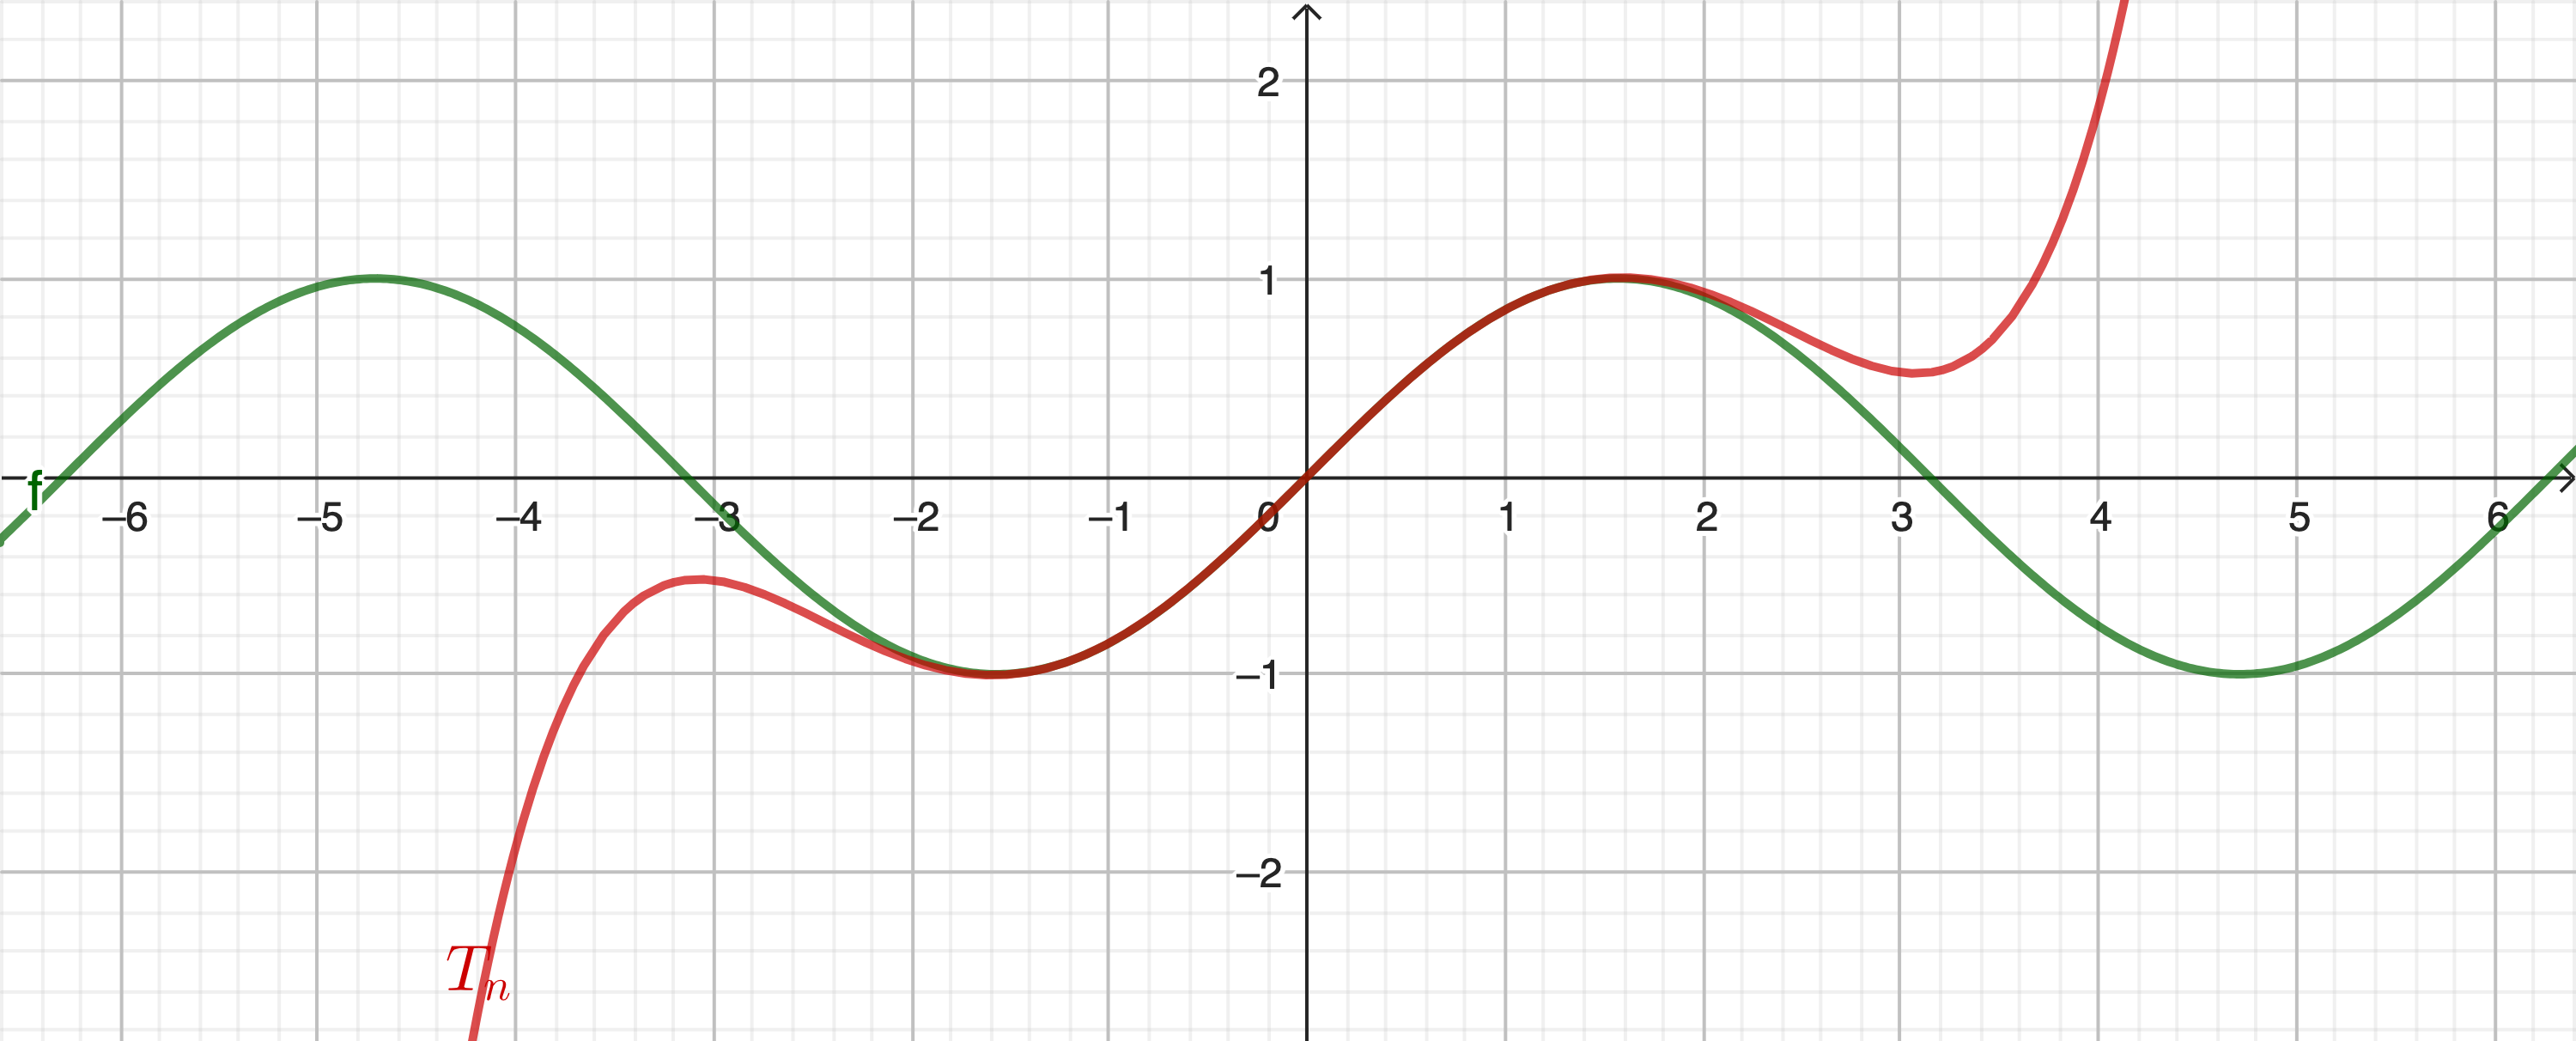
\includegraphics[width=\textwidth]{media/sinusT5.png}
		\caption*{Approximation durch ein Polynom von Grad 5}

	\end{subfigure}

\end{figure}
Die Bilder zeigen die Approximationen der Sinusfunktion durch Polynome 1., 3. und 5. Grades. Die Forderung nach weiterer Übereinstimmung in immer höheren Ableitungen führt zu immer besseren Näherungsfunktionen. Insbesondere wird der Bereich, in welchem die Taylorpolynome fast mit der Sinusfunktion übereinstimmen, immer grösser.

Wenn man diesen Prozess unendlich weiterdenkt, erhält man den folgenden Satz:
\begin{satz} {Taylorentwicklung der Sinusfunktion}{}
	$$ \sin(x) = x - \frac{1}{3!}x^3 + \frac{1}{5!}x^5 - \frac{1}{7!}x^7 + \frac{1}{9!}x^9 \pm \ldots = \sum_{k=0}^{\infty} (-1)^k \frac{x^{2k+1}}{(2k+1)!} $$
\end{satz}

Dieser Satz bildet den Schlüssel zur Berechnung von Sinuswerten unter Verwendung der vier Grundoperationen. Allerdings müsste man zur Ermittlung eines genauen Sinuswerts, unendlich viele Rechenoperationen durchführen. Deswegen verwendet man in der Praxis oft nur die ersten paar Summanden. Dabei argumentiert man wie folgt: Wenn $x$ nicht allzu gross ist, dann ist für grosse $n$  $x^n$ viel kleiner als $n!$ Also fallen die hinteren Terme der Summe  $\sum_{k=0}^{\infty} (-1)^k \frac{x^{2k+1}}{(2k+1)!}$ kaum ins Gewicht und es gilt:
$$\sin(x)\approx  x - \frac{1}{3!}x^3 + \frac{1}{5!}x^5 \qquad \text{, für $|x|$  klein} $$
Dabei gilt: Je kleiner $|x|$, desto weniger Summanden sind nötig, um eine bestimmte Genauigkeit zu erreichen und umgekehrt.

Eine solche Approximation der Sinusfunktion durch Polynome bildet die Grundidee, wie man mit dem Taschenrechner gute Näherungen für die Werte von $\sin(x)$ erzeugen kann. Allerdings verwendet der Taschenrechner in Wahrheit aus Speicher- und Laufzeitgründen eine andere, kompliziertere Methode, auf die wir hier nicht weiter eingehen werden.

Die Idee, wie wir die Sinusfunktion approximiert haben, lässt auch auf andere Funktionen anwenden:
\begin{definition}
	{Taylorpolynom}{}
	Sei $f$ eine Funktion, die an der Stelle $x_0=0$ $n$-mal differenzierbar ist. Dann nennt man
	\[
		T_n(x) = f(0) + \frac{f'(0)}{1!} \cdot x + \frac{f''(0)}{2!} \cdot x^2 + \frac{f'''(0)}{3!} \cdot x^3 + \ldots + \frac{f^{(n)}(0)}{n!} \cdot x^n = \sum_{k=0}^{n} \frac{f^{(k)}(0)}{k!} \cdot x^k
	\]
	das \emph{Taylorpolynom} $n$-ten Grades von $f$ um die Entwicklungsstelle $x_0=0$.
\end{definition}
Analog der unendliche Prozess:
\begin{definition}
	{Taylorreihe}{}
	Sei $f$ eine Funktion, die an der Stelle $x_0=0$ unendlich oft differenzierbar ist. Dann nennt man
	\[
		T(x) = f(0) + \frac{f'(0)}{1!} \cdot x + \frac{f''(0)}{2!} \cdot x^2 + \frac{f'''(0)}{3!} \cdot x^3 + \ldots = \sum_{k=0}^{\infty} \frac{f^{(k)}(0)}{k!} \cdot x^k
	\]
	die \emph{Taylorentwicklung oder die Taylorreihe} von $f$ um die Entwicklungsstelle $x_0=0$.
\end{definition}

Für jedes $x\in \R$ ist $T(x)$ eine unendliche Reihe. Jede dieser Reihen kann konvergieren oder auch nicht (siehe nächstes Kapitel).
\begin{bsp}
	{Die Taylorreihe der Sinusfunktion}{}

	Sei \( f(x) = \sin(x) \), dann gilt \[ f'(x) = \cos(x), \, f''(x) = -\sin(x) ,\, f^{(3)}(x) = -\cos(x) ,\,  f^{(4)}(x) = \sin(x) ,\, \ldots\]

	Daraus folgt wiederum, dass \[ f(0) = 0 ,\,  f'(0) = 1 ,\, f''(0) = 0 ,\,  f^{(3)}(0) = -1 ,\,  f^{(4)}(0) = 0 ,\, \ldots \]

	Damit lautet die Taylorreihe der Sinusfunktion:
	\[
		T(x) = 0 + \frac{1}{1!}x + \frac{0}{2!}x^2 - \frac{1}{3!}x^3 + \frac{0}{4!}x^4 + \ldots
		= x - \frac{x^3}{3!} + \frac{x^5}{5!} - \frac{x^7}{7!} \pm \ldots
		= \sum_{k=0}^{\infty} \frac{(-1)^k}{(2k+1)!}x^{2k+1}
	\]
\end{bsp}

Die Taylorpolynome liefern im Allgemeinen eine Approximation der Funktion in der Nähe von $x_0=0$. Durch geeignetes Verschieben kann man auch eine Näherungsfunktion an einer beliebigen anderen Stelle angeben:

\begin{definition}
	{Taylorpolynom und Taylorreihe an beliebiger Stelle}{}
	Sei \( f(x) \) eine Funktion, die an der Stelle \( x_0 \) unendlich oft differenzierbar ist. Dann nennt man

	\begin{align*}
		T_{n,x_0}(x) & = f(x_0) + \frac{f'(x_0)}{1!}(x-x_0) + \frac{f''(x_0)}{2!}(x-x_0)^2 + \ldots + \frac{f^{(n)}(x_0)}{n!}(x-x_0)^n \\
		             & = \sum_{k=0}^{n} \frac{f^{(k)}(x_0)}{k!}(x-x_0)^k
	\end{align*}

	Das Taylorpolynom \(n\)-ten Grades von \(f\) um die Entwicklungsstelle \(x_0\).

	Analog nennt man:

	\[
		T_{x_0}(x) = f(x_0) + \frac{f'(x_0)}{1!}(x-x_0) + \frac{f''(x_0)}{2!}(x-x_0)^2 + \ldots = \sum_{k=0}^{\infty} \frac{f^{(k)}(x_0)}{k!}(x-x_0)^k
	\]

	Die Taylorreihe von \(f\) um die Entwicklungsstelle \(x_0\).

\end{definition}

\begin{bsp}
	{Die Taylorreihe der Sinusfunktion um $x_0=\frac{\pi}{2}$}{}
	Sei \( f(x) = \sin(x) \). Dann gilt \( f\left(\frac{\pi}{2}\right) = 1 \), \( f'\left(\frac{\pi}{2}\right) = 0 \), \( f''\left(\frac{\pi}{2}\right) = -1 \), \( f'''\left(\frac{\pi}{2}\right) = 0 \), \( f^{(4)}\left(\frac{\pi}{2}\right) = 1 \), ...

	Daraus folgt
	\begin{align*}
		T_{\frac{\pi}{2}}(x) & = 1 + \frac{0}{1!}\left(x-\frac{\pi}{2}\right) + \frac{\left(-1\right)}{2!}\left(x-\frac{\pi}{2}\right)^2 + \frac{0}{3!}\left(x-\frac{\pi}{2}\right)^3 + \frac{1}{4!}\left(x-\frac{\pi}{2}\right)^4 + \ldots \\
		                     & = 1 - \frac{\left(x-\frac{\pi}{2}\right)^2}{2!} + \frac{\left(x-\frac{\pi}{2}\right)^4}{4!} - \frac{\left(x-\frac{\pi}{2}\right)^6}{6!} \pm \ldots                                                           \\
		                     & = \sum_{k=0}^{\infty} \frac{\left(-1\right)^k}{\left(2k\right)!}\left(x-\frac{\pi}{2}\right)^{2k}
	\end{align*}



\end{bsp}
\begin{ueb}
	{}{}

	\begin{enumerate}
		\item Bestimmen Sie die Taylorpolynome 3. Grades der folgenden Funktionen um die Entwicklungsstelle $x_0=0$. Geben Sie nach Möglichkeit auch die vollständige Taylorentwicklung mit einem Summenzeichen an:
		      \begin{enumerate}
			      \item $f(x) = \cos(x)$
			      \item $f(x)= e^x$
			      \item $f(x)= \frac{1}{1+x}=(1+x)^{-1}$
			      \item $f(x)= (x+1)^2$
			      \item $f(x)= 5x^5-7x^4+3x^3+2x+1$
		      \end{enumerate}
		\item Zeichnen Sie mit dem Computer die Graphen von $f(x)=e^x$ und von dessen Entwicklungen $T_1 (x),T_2 (x),T_3 (x)$. Verfolgen sie die wachsende Übereinstimmung.
		\item Stellen Sie die Funktion $f(x)=e^x$ als unendliche Taylorreihe dar und bestimmen Sie summandenweise die Ableitung der Reihe. Was fällt Ihnen auf?
		\item 	Betrachten Sie die Taylorreihe der Funktion $g(x)=\sin(x)$. Bestimmen Sie summandenweise die Ableitung der Reihe.
		\item Sei $v$ die Relativgeschwindigkeit zweier Inertialsysteme. Dann wird die Zeitdilatation in der SRT mit dem Lorentzfaktor berechnet:
		      \[
			      \gamma(v) = \frac{1}{\sqrt{1 - \left(\frac{v}{c}\right)^2}} = \left(1 - \frac{1}{c^2}\cdot v^2\right)^{-\frac{1}{2}}
		      \]

		      Da für Vorgänge im Alltag das Verhältnis \( \frac{v}{c} \) sehr klein ist, wird der Lorentzfaktor oft angenähert durch
		      \[
			      \gamma(v) \approx 1 + \frac{v^2}{2c^2}
		      \]

		      Zeigen Sie, dass diese Annäherung dem Taylorpolynom 2. Grades entspricht.
		      \pagebreak

		\item 	Bestimmen Sie die Taylorpolynome 3. Grades der Funktion $f$ an der Stelle $x_0$
		      \begin{enumerate}
			      \item $f(x) = \ln(x),\, x_0 = 1$
			      \item $f(x) = e^x,\, x_0 = e$
			      \item $f(x) = \cos(x),\, x_0 = \frac{\pi}{2}$
			      \item $f(x) = \sqrt{x},\, x_0 = 1$
		      \end{enumerate}
		\item 	Sei $T_{x_0}  (x)$ die Taylorentwicklung von $f$ um die Stelle $x_0$.

		      Berechnen Sie $T'(x_0 ),T'' (x_0 ),T'''(x_0 )$.
	\end{enumerate}
\end{ueb}
\clearpage

\emph{Lösungen}
\begin{enumerate}
	\item Entwicklungen
	      \begin{enumerate}
		      \item \[T_3(x) = 1-\frac{x^2}{2} , \quad T(x) = \sum_{k=0}^{\infty} \frac{(-1)^k}{(2k)!} x^{2k}\]
		      \item         \[T_3(x) = 1+x+\frac{x^2}{2!}+\frac{x^3}{3!}, \quad T(x) = \sum_{k=0}^{\infty} \frac{x^k}{k!}\]
		      \item         \[T_3(x) = 1-x+x^2-x^3, \quad T(x) = \sum_{k=0}^{\infty} (-x)^k\]
		      \item  $$T_3(x) = x^2+2x+1 = T(x) $$
		      \item         \[T_3(x) = 3x^3+2x+1, \quad T(x) = 5x^5-7x^4+3x^3+2x+1 \]
	      \end{enumerate}
	\item Grafik
	\item \[(e^x )'=(1+x+\frac{x^2}{2}+\frac{x^3}{6}+\frac{x^4}{24}+\ldots)'\]
	      \[=0+ 1+\frac{2x}{2}+\frac{3x^2}{6}+\frac{4x^3}{24}+\ldots\]
	      \[= 1+x+\frac{x^2}{2}+\frac{x^3}{6}+\ldots=e^x\]
	      Oder mit Summenformeln:
	      \[(e^x )'=\left(\sum_{k=0}^{\infty} \frac{x^k}{k!}\right)'\]
	      \[=\sum_{k=1}^{\infty} \frac{kx^{k-1}}{k!}=\sum_{k=1}^{\infty} \frac{x^{k-1}}{(k-1)!}=\sum_{k=0}^{\infty} \frac{x^k}{k!}=e^x\]
	\item \[(\sin(x) )'=(x-\frac{x^3}{6}+\frac{x^5}{120}-\frac{x^7}{5040}+\ldots)'\]
	      \[=1-\frac{3x^2}{6}+\frac{5x^4}{120}-\frac{7x^6}{5040}+\ldots\]
	      \[=1-\frac{x^2}{2}+\frac{x^4}{24}-\frac{x^6}{720}+\ldots=\cos(x)\]
	      Oder mit Summenformeln:
	      \[\left(\sum_{k=0}^{\infty} \frac{(-1)^k}{(2k+1)!} x^{2k+1}\right)'\]
	      \[=\sum_{k=0}^{\infty} \frac{(2k+1)(-1)^k}{(2k+1)!} x^{2k}=\sum_{k=0}^{\infty} \frac{(-1)^k}{(2k)!} x^{2k}=\cos(x)\]
	\item Einige Zwischenresultate:

	      $ \gamma'(v) = \frac{v}{c^2}\cdot \left(1-\frac{v^2}{c^2}\right)^{-\frac{3}{2}}  $ und $\gamma''(v) = \frac{1}{c^2}\cdot \left(1-\frac{v^2}{c^2}\right)^{-\frac{3}{2}} + \frac{3v^2}{c^4} \left(1-\frac{v^2}{c^2}\right)^{-\frac{5}{2}} $


	      % \[\gamma(v)\approx 1+\frac{v^2}{2c^2} \]
	\item Taylor an anderer Stelle
	      \begin{enumerate}
		      \item \[(x-1)-\frac{(x-1)^2}{2}+\frac{(x-1)^3}{3}\]
		      \item \[e^e+e^e (x-e)+\frac{e^e}{2} (x-e)^2+\frac{e^e}{3!} (x-e)^3\]
		      \item \[-(x-\frac{\pi}{2})+\frac{(x-\frac{\pi}{2})^3}{6}\]
		      \item
		            \[1+\frac{(x-1)}{2}-\frac{(x-1)^2}{8}+\frac{(x-1)^3}{16}\]

	      \end{enumerate}
	\item
	      \[T'(x_0)=f'(x_0), T''(x_0)=f''(x_0), T'''(x_0)=f'''(x_0), \ldots\]

\end{enumerate}

\begin{satz}
	{Diese Taylorreihen sollten Sie auswendig lernen}{}

	\begin{align*}
		\sin(x) & = x - \frac{x^3}{3!} + \frac{x^5}{5!} - \frac{x^7}{7!} \pm \ldots = \sum_{k=0}^{\infty} \frac{(-1)^k}{(2k+1)!} x^{2k+1} \\
		\cos(x) & = 1 - \frac{x^2}{2!} + \frac{x^4}{4!} - \frac{x^6}{6!} \pm \ldots = \sum_{k=0}^{\infty} \frac{(-1)^k}{(2k)!} x^{2k}     \\
		e^x     & = 1 + \frac{x}{1!} + \frac{x^2}{2!} + \frac{x^3}{3!} + \ldots = \sum_{k=0}^{\infty} \frac{x^k}{k!}
	\end{align*}

\end{satz}















